% !TEX root = robobrain.tex
\subsubsection{Path planning using \robobrain{}}
\label{sec:applicationplanit}

One key problem robots face in performing tasks in human environments is identifying trajectories desirable to the users. An appropriate trajectory not only needs to be valid from a geometric standpoint (i.e., feasible and obstacle-free), but it also needs to satisfy the user preferences~\citep{jainsaxena2013_trajectorypreferences,Jain14}. For example,  a robot should move sharp objects such as knife strictly away from nearby humans~\cite{jain_contextdrivenpathplanning_2013}. Such preferences are commonly represented as cost functions which jointly model the environment, the task, and trajectories.
%This joint modeling is expensive in terms of resource requirement (e.g., robots) and data collection, and
Typically research groups have independently learned different cost functions~\citep{jainsaxena2013_trajectorypreferences,Kuderer-RSS-12,KitaniECCV2012}, which are not shared across the research groups. Here we show \robobrain{} \textit{as-a-service}  for a robot to store and retrieve the planning parameters.
%We now show how the previous work by Jain et al.~\citep{Jain14} use the RKE for retrieving the trajectory parameters for path planning. We demonstrate this on the example of moving an egg carton from the previous work~\citep{Jain14}.

In Figure~\ref{fig:planning} we illustrate the robot planning for an egg carton by querying \robobrain{}.
Since eggs are \textit{fragile}, users  prefer to move them slowly and close to the surface of the table.  In order to complete the task, the robot queries \robobrain{} and retrieves the attributes of the egg carton and also the trajectory parameters learned in the previous work by Jain et al.~\citep{Jain14}. Using the retrieved attributes and the parameters, the robot samples trajectories and executes the top-ranked trajectory.
%need labels of all objects in the environment. In this example we use the
%object labels provided by the authors~\cite{Jain14}. After the object labels are obtained, the previous
%work~\citep{Jain14} use the RKE to retrieve attributes of the egg carton and also the trajectory
%parameters.
Below we show the RQL queries.
%\noindent \resizebox{\linewidth}{!}{
%\begin{minipage}{\linewidth}
{\small
\begin{align*}
&{\tt {attributes} \,\, n := fetch \,\,(\{name:n\})\rightarrow
[`HasAttribute'] \rightarrow (v)   \nonumber} \\
&{\tt {trajectories} \,\, a := }\\
&{\tt\hspace*{2cm} fetch \,(\{handle :a\})\rightarrow  [`HasTrajectory'] \rightarrow (v)  \nonumber } \\
&{\tt {trajectory\_parameters} := }\\
&{\tt \hspace*{2cm} map (\lambda a \rightarrow
{trajectories}\,\, a)  \,\, {attributes}\,\, `egg' } \nonumber
\end{align*}
%  \end{minipage}
}

\begin{figure}[t]
\centering
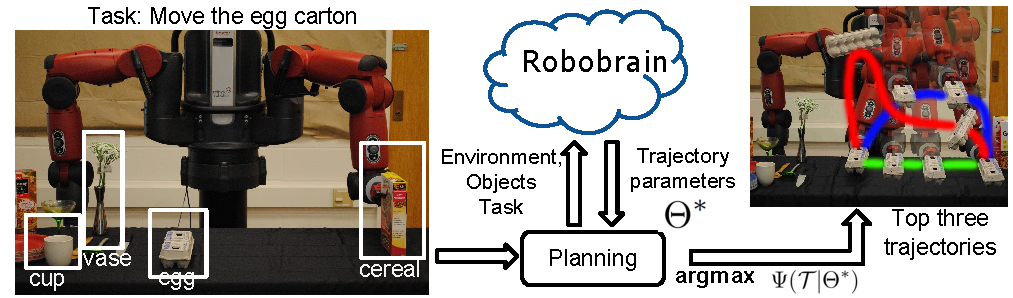
\includegraphics[width=\linewidth]{Image/planit_robobrain_pic_2}
\caption{\textbf{\robobrain{} for planning trajectory.} The robot queries \robobrain{} for the trajectory parameters (learned by Jain et al.~\citep{jainsaxena2013_trajectorypreferences})  to plan paths for the fragile objects like an egg carton. }
\label{fig:planning}
\end{figure}
